% questions.tex —— 2009 年·普通高等学校招生考试·湖北卷·理科 · 题目内容片段（无答案）
% 由 tools/generate_projects.py 依来源总账自 2009/2009_数学真题_湖北理_试题.md 生成，勿手改（改源 MD 后重跑）


状态：needs-review；依固定候选 PDF 两页（印刷页 523–524）逐题核验，图形已矢量重绘。原页未印分值，不补。

\gkpart{一、选择题}

\begin{question}
\gkti{1}已知 $P=\{\boldsymbol a\mid\boldsymbol a=(1,0)+m(0,1),\ m\in\mathbf R\}$，$Q=\{\boldsymbol b\mid\boldsymbol b=(1,1)+n(-1,1),\ n\in\mathbf R\}$ 是两个向量集合，则 $P\cap Q=$（　）

（A）$\{(1,1)\}$

（B）$\{(-1,1)\}$

（C）$\{(1,0)\}$

（D）$\{(0,1)\}$

\end{question}
\begin{question}
\gkti{2}函数 $y=\dfrac{1-ax}{1+ax}$（$x\in\mathbf R$，$x\neq-\dfrac1a$）的反函数是（　）

（A）$y=\frac{1-ax}{1+ax}$（$x\in\mathbf R$，$x\neq-\frac1a$）

（B）$y=\frac{1+ax}{1-ax}$（$x\in\mathbf R$，$x\neq\frac1a$）

（C）$y=\frac{1+x}{a(1-x)}$（$x\in\mathbf R$，$x\neq1$）

（D）$y=\frac{1-x}{a(1+x)}$（$x\in\mathbf R$，$x\neq-1$）

\end{question}
\begin{question}
\gkti{3}投掷两颗骰子，得到其向上的点数分别为 $m$ 和 $n$，则复数 $(m+n\mathrm i)(n-m\mathrm i)$ 为实数的概率为（　）

（A）$\frac13$

（B）$\frac14$

（C）$\frac16$

（D）$\frac1{12}$

\end{question}
\begin{question}
\gkti{4}函数 $y=\cos\left(2x+\dfrac\pi6\right)-2$ 的图象 $F$ 按向量 $\boldsymbol a$ 平移到 $F'$，$F'$ 的解析式 $y=f(x)$，当 $y=f(x)$ 为奇函数时，向量 $\boldsymbol a$ 可以等于（　）

（A）$\left(-\frac\pi6,-2\right)$

（B）$\left(-\frac\pi6,2\right)$

（C）$\left(\frac\pi6,-2\right)$

（D）$\left(\frac\pi6,2\right)$

\end{question}
\begin{question}
\gkti{5}将甲、乙、丙、丁四名学生分到三个不同的班，每个班至少分到一名学生，且甲、乙两名学生不能分到一个班，则不同分法的种数为（　）

（A）$18$

（B）$24$

（C）$30$

（D）$36$

\end{question}
\begin{question}
\gkti{6}设 $\left(\dfrac{\sqrt2}{2}+x\right)^{2n}=a_0+a_1x+a_2x^2+\cdots+a_{2n-1}x^{2n-1}+a_{2n}x^{2n}$，则

\nopagebreak[4]
\[\lim_{n\to\infty}\left[(a_0+a_2+a_4+\cdots+a_{2n})^2-(a_1+a_3+a_5+\cdots+a_{2n-1})^2\right]=\]

（　）

（A）$-1$

（B）$0$

（C）$1$

（D）$\frac{\sqrt2}{2}$

\end{question}
\begin{question}
\gkti{7}已知双曲线 $\dfrac{x^2}{2}-\dfrac{y^2}{2}=1$ 的准线过椭圆 $\dfrac{x^2}{4}+\dfrac{y^2}{b^2}=1$ 的焦点，则直线 $y=kx+2$ 与椭圆至多有一个交点的充要条件是（　）

（A）$k\in\left[-\frac12,\frac12\right]$

（B）$k\in\left(-\infty,-\frac12\right]\cup\left[\frac12,+\infty\right)$

（C）$k\in\left[-\frac{\sqrt2}{2},\frac{\sqrt2}{2}\right]$

（D）$k\in\left(-\infty,-\frac{\sqrt2}{2}\right]\cup\left[\frac{\sqrt2}{2},+\infty\right)$

\end{question}
\begin{question}
\gkti{8}在“家电下乡”活动中，某厂要将 $100$ 台洗衣机运往邻近的乡镇，现有 $4$ 辆甲型货车和 $8$ 辆乙型货车可供使用，每辆甲型货车运输费用 $400$ 元，可装洗衣机 $20$ 台；每辆乙型货车运输费用 $300$ 元，可装洗衣机 $10$ 台，若每辆至多只运一次，则该厂所花的最少运输费用为（　）

（A）$2000$ 元

（B）$2200$ 元

（C）$2400$ 元

（D）$2800$ 元

\end{question}
\begin{question}
\gkti{9}设球的半径为时间 $t$ 的函数 $R(t)$．若球的体积以均匀速度 $c$ 增长，则球的表面积的增长速度与球半径（　）

（A）成正比，比例系数为 $c$

（B）成正比，比例系数为 $2c$

（C）成反比，比例系数为 $c$

（D）成反比，比例系数为 $2c$

\Needspace{0.4\textheight}
\end{question}
\begingroup
\renewenvironment{question}{\Needspace{0.5\textheight}}{}
\begin{question}
\gkti{10}古希腊人常用小石子在沙滩上摆成各种性状来研究数，例如：
\nopagebreak[4]
\begin{center}% 2009 年湖北卷理科第 10 题：三角形数与正方形数的点阵图（图 1、图 2）。
% 来源 PDF：2009湖北理.pdf，SHA-256 a78cef31900f38a49e4940931067c750cdff63c9d4dab40c72dbd09e56e80f3a。
% 原页：第 1 页第 2 栏中部，书页码 523。
% 重绘依据：按原页逐点重绘，点数与排列照原页。
%   图 1：三角形数 1、3、6、10，自下而上每行比下一行少一点且逐行居中（1+2+3+4 点）。
%   图 2：正方形数 1、4、9、16，为 1×1、2×2、3×3、4×4 的方阵，各组底边对齐。
%   两组末均以省略号表示后续。
\begin{tikzpicture}[x=0.46cm, y=0.46cm, semithick,
  every node/.style={inner sep=1pt, font=\small}]

  % ---------- 图 1：三角形数 ----------
  % 1
  \fill (0,0) circle (2.1pt);
  % 3
  \fill (2.4,0) circle (2.1pt);
  \fill (3.4,0) circle (2.1pt);
  \fill (2.9,1) circle (2.1pt);
  % 6
  \fill (5.8,0) circle (2.1pt);
  \fill (6.8,0) circle (2.1pt);
  \fill (7.8,0) circle (2.1pt);
  \fill (6.3,1) circle (2.1pt);
  \fill (7.3,1) circle (2.1pt);
  \fill (6.8,2) circle (2.1pt);
  % 10
  \fill (10.2,0) circle (2.1pt);
  \fill (11.2,0) circle (2.1pt);
  \fill (12.2,0) circle (2.1pt);
  \fill (13.2,0) circle (2.1pt);
  \fill (10.7,1) circle (2.1pt);
  \fill (11.7,1) circle (2.1pt);
  \fill (12.7,1) circle (2.1pt);
  \fill (11.2,2) circle (2.1pt);
  \fill (12.2,2) circle (2.1pt);
  \fill (11.7,3) circle (2.1pt);

  \node at (14.7,1.4) {$\cdots$};
  \node[below] at (0,-0.6) {$1$};
  \node[below] at (2.9,-0.6) {$3$};
  \node[below] at (6.8,-0.6) {$6$};
  \node[below] at (11.7,-0.6) {$10$};
  \node at (7.3,-2.55) {图 1};

  % ---------- 图 2：正方形数 ----------
  \begin{scope}[yshift=-3.5cm]
    % 1
    \fill (0,0) circle (2.1pt);
    % 4
    \fill (2.4,0) circle (2.1pt);
    \fill (3.4,0) circle (2.1pt);
    \fill (2.4,1) circle (2.1pt);
    \fill (3.4,1) circle (2.1pt);
    % 9
    \foreach \i in {5.8,6.8,7.8} {
      \foreach \j in {0,1,2} {
        \fill (\i,\j) circle (2.1pt);
      }
    }
    % 16
    \foreach \i in {10.2,11.2,12.2,13.2} {
      \foreach \j in {0,1,2,3} {
        \fill (\i,\j) circle (2.1pt);
      }
    }

    \node at (14.7,1.4) {$\cdots$};
    \node[below] at (0,-0.6) {$1$};
    \node[below] at (2.9,-0.6) {$4$};
    \node[below] at (6.8,-0.6) {$9$};
    \node[below] at (11.7,-0.6) {$16$};
    \node at (7.3,-2.55) {图 2};
  \end{scope}
\end{tikzpicture}
\end{center}
\nopagebreak[4]
他们研究过图 1 中的 $1$，$3$，$6$，$10$，$\cdots$，由于这些数能够表示成三角形，将其称为三角形数；类似地，称图 2 中的 $1$，$4$，$9$，$16\cdots$ 这样的数成为正方形数．下列数中及时三角形数又是正方形数的是（　）

（A）$289$

（B）$1024$

（C）$1225$

（D）$1378$

\end{question}
\endgroup
\gkpart{二、填空题}

\begin{question}
\gkti{11}已知关于 $x$ 的不等式 $\dfrac{ax-1}{x+1}<0$ 的解集是 $(-\infty,-1)\cup\left(-\dfrac12,+\infty\right)$，则 $a=$\gkblank{}．

\Needspace{0.4\textheight}
\end{question}
\begingroup
\renewenvironment{question}{\Needspace{0.4\textheight}}{}
\begin{question}
\gkti{12}样本容量为 $200$ 的频率分布直方图．根据样本的频率分布直方图估计，样本数据落在 $[6,10)$ 内的频数为\gkblank{}，数据落在 $[2,10)$ 内的概率约为\gkblank{}．
\nopagebreak[4]
\begin{center}% 2009 年湖北卷理科第 12 题：样本容量 200 的频率分布直方图。
% 来源 PDF：2009湖北理.pdf，SHA-256 a78cef31900f38a49e4940931067c750cdff63c9d4dab40c72dbd09e56e80f3a。
% 原页：第 1 页第 2 栏中部，书页码 523。
% 重绘依据：横轴 0—22，0 与 2 之间为省略断轴；纵轴为「频率/组距」，组距 4。
%   五组矩形高：[2,6)=0.02，[6,10)=0.08，[10,14)=0.09，[14,18)=0.03，[18,22)=0.03；
%   0.02+0.08+0.09+0.03+0.03=0.25，乘组距 4 恰为 1，已核对。
%   虚线标出 0.02、0.03、0.08、0.09 四条水平参考线，位置照原页。
%   原页原点刻度标「0」而非「O」，按原页照录。
\begin{tikzpicture}[x=0.34cm, y=30cm, semithick,
  every node/.style={inner sep=1.2pt, font=\small}]

  % 水平虚线参考线（画在矩形之下，白色填充的矩形覆盖其内部）
  \draw[dashed] (0,0.09) -- (10,0.09);
  \draw[dashed] (0,0.08) -- (10,0.08);
  \draw[dashed] (10,0.03) -- (22,0.03);
  \draw[dashed] (0,0.02) -- (2,0.02);

  % 各组矩形
  \draw[fill=white] (2,0) rectangle (6,0.02);
  \draw[fill=white] (6,0) rectangle (10,0.08);
  \draw[fill=white] (10,0) rectangle (14,0.09);
  \draw[fill=white] (14,0) rectangle (18,0.03);
  \draw[fill=white] (18,0) rectangle (22,0.03);

  % 坐标轴
  \draw[-{Stealth}] (-0.5,0) -- (23.4,0) node[right, inner sep=3pt] {样本数据};
  \draw[-{Stealth}] (0,-0.002) -- (0,0.1125);
  \node[anchor=west] at (0.45,0.1045) {频率/组距};

  % 断轴符号（0 与 2 之间）
  \draw (0.45,0) -- (0.58,0.0022) -- (0.71,0) -- (0.84,0.0022) -- (0.97,0);

  % 刻度与标签
  \foreach \x in {2,6,10,14,18,22} {
    \draw (\x,0) -- (\x,-0.0012);
    \node[below] at (\x,-0.0018) {$\x$};
  }
  \node[below left=1pt] at (0,0) {$0$};

  % 纵轴刻度标签
  \foreach \h/\t in {0.02/0.02, 0.03/0.03, 0.08/0.08, 0.09/0.09} {
    \node[left, font=\scriptsize] at (0,\h) {\t};
  }
\end{tikzpicture}
\end{center}
\nopagebreak[4]
\end{question}
\endgroup
\begin{question}
\gkti{13}卫星和地面之间的电视信号沿直线传播，电视信号能够传送到达的地面区域，称为这个卫星的覆盖区域．为了转播 $2008$ 年北京奥运会，我国发射了“中星九号”广播电视直播卫星，它离地球表面的距离约为 $36000\ \mathrm{km}$．已知地球半径约为 $6400\ \mathrm{km}$，则“中星九号”覆盖区域内的任意两点的球面距离的最大值约为\gkblank{}$\mathrm{km}$．（结果中保留反余弦的符号）

\end{question}
\begin{question}
\gkti{14}已知函数 $f(x)=f'\left(\dfrac\pi4\right)\cos x+\sin x$，则 $f\left(\dfrac\pi4\right)$ 的值为\gkblank{}．

\end{question}
\begin{question}
\gkti{15}已知数列 $\{a_n\}$ 满足：$a_1=m$（$m$ 为正整数），$a_{n+1}=\begin{cases}\dfrac{a_n}{2},& \text{\text{当} } a_n \text{ \text{为偶数时}},\\[4pt] 3a_n+1,& \text{\text{当} } a_n \text{ \text{为奇数时}}.\end{cases}$ 若 $a_6=1$，则 $m$ 所有可能的取值为\gkblank{}．

\end{question}
\gkpart{三、解答题}

\begin{question}
\gkti{16}一个盒子里装有 $4$ 张大小形状完全相同的卡片，分别标有数 $2$，$3$，$4$，$5$；另一个盒子也装有 $4$ 张大小形状完全相同的卡片，分别标有数 $3$，$4$，$5$，$6$．现从一个盒子中任取一张卡片，其上面的数记为 $x$；再从另一盒子里任取一张卡片，其上面的数记为 $y$，记随机变量 $\eta=x+y$，求 $\eta$ 的分布列和数学期望．

\end{question}
\begin{question}
\gkti{17}已知向量 $\boldsymbol a=(\cos\alpha,\sin\alpha)$，$\boldsymbol b=(\cos\beta,\sin\beta)$，$\boldsymbol c=(-1,0)$．

（1）求向量 $\boldsymbol b+\boldsymbol c$ 的长度的最大值；

（2）设 $\alpha=\dfrac\pi4$，且 $\boldsymbol a\perp(\boldsymbol b+\boldsymbol c)$，求 $\cos\beta$ 的值．

\Needspace{0.4\textheight}
\end{question}
\begingroup
\renewenvironment{question}{\Needspace{0.5\textheight}}{}
\begin{question}
\gkti{18}如图，四棱锥 $S-ABCD$ 的底面是正方形，$SD\perp$ 平面 $ABCD$，$SD=2a$，$AD=\sqrt2a$，点 $E$ 是 $SD$ 上的点，且 $DE=\lambda a$（$0<\lambda\leqslant2$）．

（1）求证：对任意的 $\lambda\in(0,2]$，都有 $AC\perp BE$；

（2）设二面角 $C-AE-D$ 的大小为 $\theta$，直线 $BE$ 与平面 $ABCD$ 所成的角为 $\varphi$．若 $\tan\theta\cdot\tan\varphi=1$，求 $\lambda$ 的值．
\nopagebreak[4]
\begin{center}% 2009 年湖北卷理科第 18 题：四棱锥 S-ABCD。
% 来源 PDF：2009湖北理.pdf，SHA-256 a78cef31900f38a49e4940931067c750cdff63c9d4dab40c72dbd09e56e80f3a。
% 原页：第 2 页第 1 栏上部，书页码 524。
% 重绘依据：底面 ABCD 为正方形，SD⊥底面，故 SD 画成竖直线并落到底面顶点 D 上；
%   D 在锥体内部，SD、DA、DC、AC 均被遮挡，画虚线；SA、SB、SC、AB、BC 为可见
%   棱，画实线。原页未在图上标出点 E（E 在 SD 上，由题面给出 DE=λa），故此处亦
%   不添标 E，保持与原页一致。
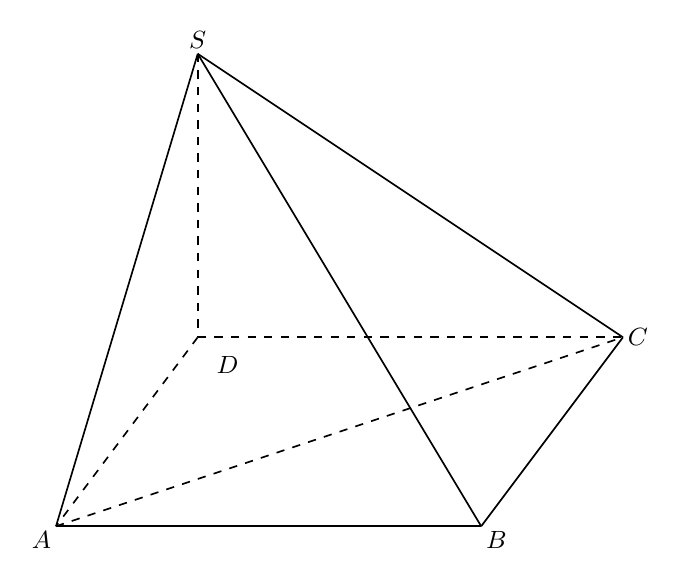
\begin{tikzpicture}[semithick, every node/.style={inner sep=1.5pt, font=\small}]
  \coordinate (A) at (0.2,1.2);
  \coordinate (B) at (5.6,1.2);
  \coordinate (C) at (7.4,3.6);
  \coordinate (D) at (2.0,3.6);
  \coordinate (S) at (2.0,7.2);

  % 可见棱
  \draw (S) -- (A);
  \draw (S) -- (B);
  \draw (S) -- (C);
  \draw (A) -- (B);
  \draw (B) -- (C);

  % 被遮挡的棱
  \draw[dashed] (S) -- (D);
  \draw[dashed] (D) -- (A);
  \draw[dashed] (D) -- (C);
  \draw[dashed] (A) -- (C);

  % 标签
  \node[above] at (S) {$S$};
  \node[below right=5pt] at (D) {$D$};
  \node[below left] at (A) {$A$};
  \node[below right] at (B) {$B$};
  \node[right] at (C) {$C$};
\end{tikzpicture}
\end{center}
\nopagebreak[4]
\end{question}
\endgroup
\begin{question}
\gkti{19}已知 $\{a_n\}$ 的前 $n$ 项和 $S_n=-a_n-\left(\dfrac12\right)^{n-1}+2$（$n$ 为正整数）．

（1）令 $b_n=2^na_n$，求证数列 $\{b_n\}$ 是等差数列，并求数列 $\{a_n\}$ 的通项公式；

（2）令 $c_n=\dfrac{n+1}{n}a_n$，$T_n=c_1+c_2+\cdots+c_n$，试比较 $T_n$ 与 $\dfrac{5n}{2n+1}$ 的大小，并予以证明．

\end{question}
\begin{question}
\gkti{20}过抛物线 $y^2=2px$（$p>0$）的对称轴上一点 $A(a,0)$（$a>0$）的直线与抛物线相交于 $M$、$N$ 两点，自 $M$、$N$ 向直线 $l:x=-a$ 作垂线，垂足分别为 $M_1$、$N_1$．

（1）当 $a=\dfrac p2$ 时，求证：$AM_1\perp AN_1$；

（2）记 $\triangle AMM_1$、$\triangle AM_1N_1$、$\triangle ANN_1$ 的面积分别为 $S_1$、$S_2$、$S_3$，是否存在 $\lambda$，使得对任意的 $a>0$，都有 $S_2^2=\lambda S_1S_3$ 成立．若存在，求出 $\lambda$ 的值；若不存在，说明理由．

\end{question}
\begin{question}
\gkti{21}在 $\mathbf R$ 上定义运算 $\otimes$：$p\otimes q=-\dfrac13(p-c)(q-b)+4bc$（$p$、$q$ 为实常数）．记 $f_1(x)=x^2-2c$，$f_2(x)=x-2b$，$x\in\mathbf R$．令 $f(x)=f_1(x)\otimes f_2(x)$．

（1）如果函数 $f(x)$ 在 $x=1$ 处有极值 $-\dfrac43$，试确定 $b$、$c$ 的值；

（2）求曲线 $y=f(x)$ 上斜率为 $c$ 的切线与该曲线的公共点；

（3）记 $g(x)=|f'(x)|$（$-1\leqslant x\leqslant 1$）的最大值为 $M$．若 $M\geqslant k$ 对任意的 $b$、$c$ 恒成立，试求 $k$ 的最大值．

\end{question}